\documentclass[12pt]{article}
\usepackage{
  amsmath,
  booktabs,
  enumitem,
  geometry,
  graphicx,
  microtype,
  parskip,
}
\geometry{margin=3cm}

% meta data
\newcommand{\chapter}{2.3}
\newcommand{\authorname}{Amo DelBello}
\newcommand{\classdescription}{MATH 1350-D2}
\newcommand{\classname}{Introduction to Statistics, Fall 2022}
\newcommand{\assignment}{\chapter\ Book Assignment}

\newcommand{\problem}[1]{\vspace{5ex}\section*{\chapter-#1}}
\newcommand{\thead}[1]{\textnormal{\textbf{#1}}}
\newcommand{\tvspace}{\vspace{.25cm}}

\title{\classdescription\ \\ \classname\ \\ $\ $ \\ \assignment}
\author{\authorname}
\date{\today}


\begin{document}
\maketitle

\problem{2}
No. Choosing to use a graph to present the data has no effect on the quality of the data or how it was obtained.


\problem{5}
Yes, there appears to be an outlier with a value of 36.

\pagebreak
\problem{10}
\begin{figure}[ht]
  \centering
  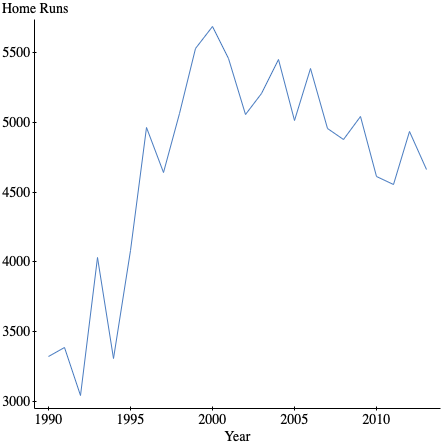
\includegraphics[width=12cm]{assets/home-runs.png}
  \caption{MLB Home Runs per Year}
\end{figure}

There appears to be a trend of steadily increasing totals until around the year 2000 and then a slight drop in the following years. Overall, this graph appears to show a normal distribution skewed to the right.


\pagebreak
\problem{14}
\begin{figure}[ht]
  \centering
  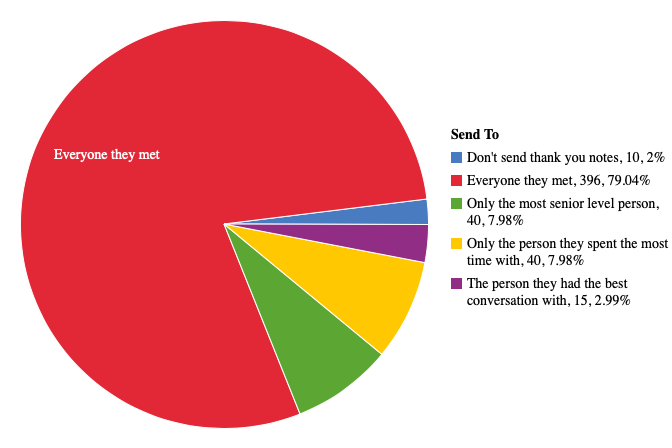
\includegraphics[width=14cm]{assets/job-interview-notes.png}
  \caption{Sending Followup Interview Thank-You Notes}
\end{figure}

\pagebreak
\problem{16}
\begin{figure}[ht]
  \centering
  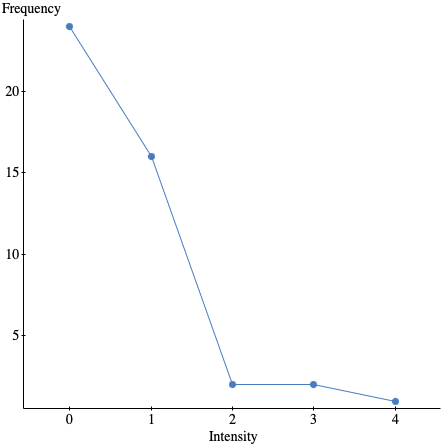
\includegraphics[width=12cm]{assets/tornado-intensity.png}
  \caption{Frequency of Tornado Intensity}
\end{figure}

The graph suggests that the data is skewed to the right.


\problem{18}
The graph is deceptive because it multiplies both the height and the width by 2.5. This results in a  ``Current Subway Fare'' graphic that is 6.25 times larger than the ``1986 Subway Fare'' graphic instead of 2.5 times larger.


\problem{20}
The graph is deceptive because all three dimensions (height, width, and depth) are multiplied by the differences in incomes, resulting in much larger differences in the sizes of the graphics than differences in incomes levels for the respective degrees.


\end{document}
%%% Local Variables:
%%% mode: latex
%%% TeX-master: t
%%% End:
